
\section{Introdução}

\lipsum[2-4]

\section{Algoritmos}

\begin{algorithm}[H]
  \SetAlgoLined %APAGAR
  \KwData{Entrada do algoritimo}
  \KwIn{entrada} \
   \KwResult{Resultado do codigo} \
   \While{$x = 0$}{
    Leia atual \;
    \eIf{$n = 2$}{
     vá para aproxima seção \;
     a seção atual se torna esta \;
     }{
     VOlta ao inicio da seção \;
      \Return{EXIT}
    }
   }
   \caption{Nome do algoritimo em Portugues}


\end{algorithm}

\section{Qr CODE}
\par Exemplo de acição de QRcode.
\qrcode {https://dicionario.priberam.org/}
\qquad
QrCode com 5cm:
\quad
\qrcode[height=5cm]{https://github.com/OgliariNatan/Template-UNOPAR}

\subsection{Dicionário}

\par Sugiro este dicionário, para dividas quanto a línga.
\quad
\qrcode {https://dicionario.priberam.org/}

\section{Código externo no main.c}

\lstinputlisting[language=c]{main.c} %Busca os codigos na pasta /cod

\subsection{Banco de dados} \label{Banco de dados}

$\underline{{\color{Blue} }}{\color{red} \, \: \: \left ( \iint_{\widetilde{ \theta }}^{\phi } \right )}  $

\lipsum[2-4]

\subsection{Algoritmo}
\par Um exemplo de adição de Algoritmo. \\

\begin{algorithm}[H]
  \caption{Calculo da potênciação.}
  \label{ap1.2}
  \Entrada{a, b, valor}
  \Saida{Valor da potênciação}
  Var \\
  a, b, valor: inteiro; \Comment {Declara as variável do tipo inteiro.}

  \Inicio{
    escreva ("Você deverá entrar com dois valores, sendo que eles deverão ser
    positivos e inteiros.") \Comment {Inicio do algoritmo.} \\
    escreva ("") \\
    escreva ("Entre com o valor de a:") \\
    leia (a) \\
    escreva("Entre com o valor de b:") \\
    leia(b) \\
    $valor \leftarrow 1$ \\
    \While{$b \neq 0$}{
      $valor  \leftarrow  a  \times valor$ \\
      $b \leftarrow b-1$
    }
    escreval ("A Potência é:", valor)
    }
\end{algorithm}

\section{Resultados e discussões}
%%%%%%%%%%%%%%%%%%%%%%%%%%%%%%%%%%%%%%%%%%%%%%%

\par Aqui vai um exemplo de código em \LaTeX2e.

\begin{algorithm} [H]
	\caption{O nome do código}\label{alg:cap}

	\begin{algorithmic} [H]
		\Require $n \geq 0$	\Comment {n será maior ou igual a zero.}
    \Require $x \geq 10$	\Comment {x será maior que 10.}
		\Ensure $y = x^n$   	\Comment {adicionado.}
    \Ensure $x = n $      \Comment{Idiota.}
		\State $y \gets 1$
		\State $X \gets x$
		\State $N \gets n$
%		\While{$N \neq 0$}
%			\If{$N$ is even}
%			 	   \State $X \gets X \times X$
% 			   	\State $N \gets \frac{N}{2}$  \Comment{Aqui Vai o meu comentario}
%			\ElsIf{$N = 0$ }
%   				 \State $y \gets y \times X$
%  			 	 \State $N \gets N - 1$
%				\State $Xold \gets Xnew$
%			\EndIf
%		\EndWhile
	\end{algorithmic}

\end{algorithm}

\section{Sub Figuras}

\begin{figure}[H] %Figuras da aula pratica 1.1
  \center
  \subfigure[ Algoritmo.\label{fig:pri2}]{
\includegraphics[scale=0.4]{figure/placeholder.jpg}}
  \subfigure[Comportamento.\label{fig:seg2}]{
\includegraphics[scale=.4]{figure/placeholder.jpg}}
  \caption{Resultado da atividade prática 1.2}\label{fig:ap1_cod_vigual1}
\end{figure}

%%%%%%%%%%%%%%%%%%%%%%%%%%%%%%%%%%%%%%%%%%%%%%%%%%%%%%%%%%
\section{Seção que será apagada}

Para referenciar utilize \cite{ninguem2022curioso}. Também pode ser citado integrada ao texto, de acordo com \citeonline{alguem2022nada}.

Para inserir imagens adicione a figura no diretório \textit{/figure}

\begin{figure}[H]
\centering
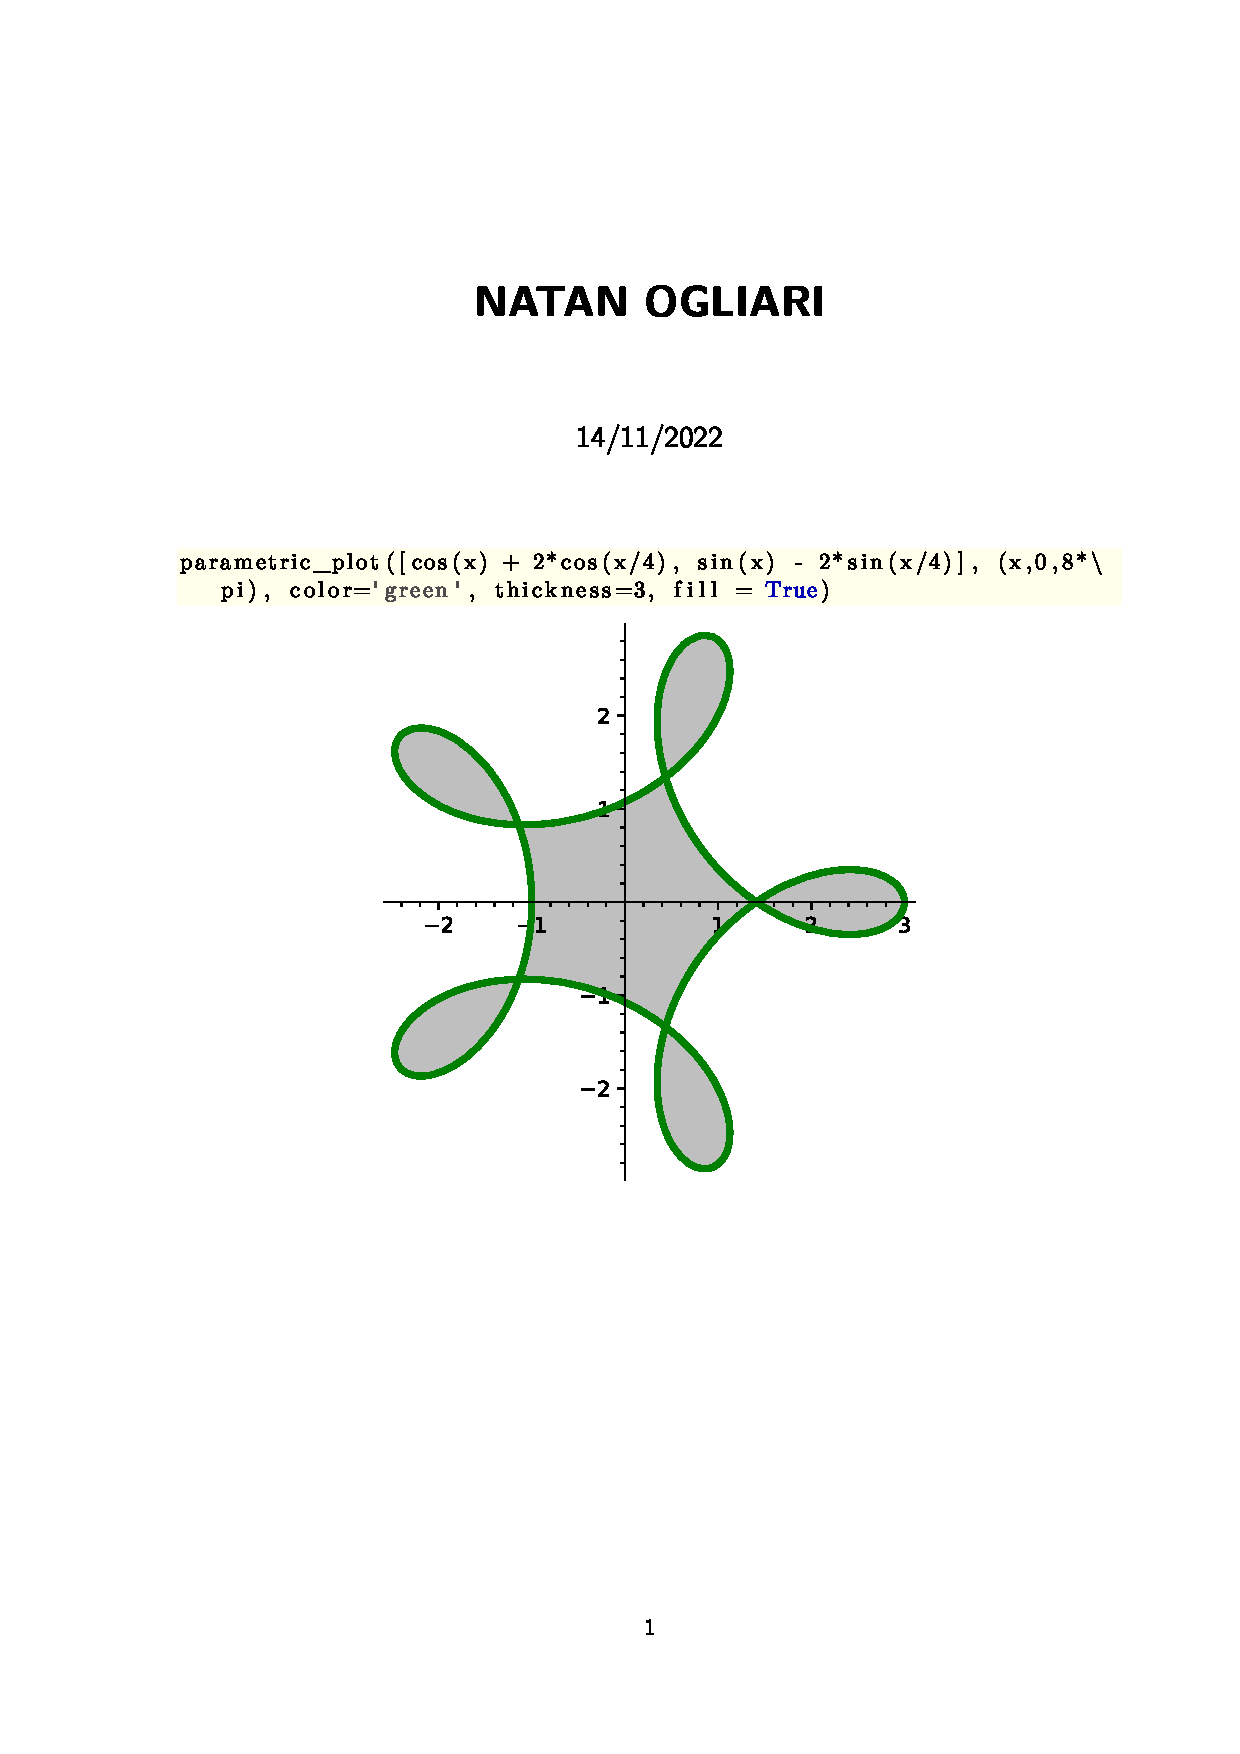
\includegraphics[width=1\textwidth]{figure/Welcome to CoCalc.pdf}
\caption{Exemplo de uma imagem bem massa aqui}
\label{fig:imagem_massa}
\end{figure}

\par Estou usando \href {https://cocalc.com/} {CoCal}

E para referenciar a figura \ref{fig:imagem_massa} utilize dessa forma.




\par Exemplo de incerção de formula, $ \sqrt{x} + \sqrt{\smash[b]{y}} + \sqrt{z} $


$\sum_{n<k,\;\text{$n$ odd}} nE_n$

\section{Sub itens}

\begin{enumerate}[label=\Roman{*}, ref=(\roman{*})]
  \item fsfsdf
  \item kugfhiuh
\end{enumerate}

\begin{asparaenum}
\item Every ...
\item The next ... \label{pl1}
\end{asparaenum}


\section{Conclusões}

\begin{algorithm}
\DontPrintSemicolon
\KwData{Ponteiros randomicos.} \Comment{Testando meu comentario} \\
\KwResult{Ordenação de vetores, e concatenação de vetores.}

\Begin{ \Comment{Inicio do meu algoritimo.} \\
$V \longleftarrow X$\;
$S \longleftarrow \emptyset$\;
\For{$x\in X$}{
  $NbSuccInS(x) \longleftarrow 0$\;
  $NbPredInMin(x) \longleftarrow 0$\;
  $NbPredNotInMin(x) \longleftarrow |ImPred(x)|$\;
}
\For{$x \in X$}{
  \If{$ponteiroValido() = 1$ {\bf and} $filaVazia() = 1$}{
    $SOMA4()$}
    }
\nl\While{$S \neq \emptyset$}{\label{InRes1}
\nlset{REM} remove $x$ from the list of $T$ of maximal index\;\label{InResR}
\lnl{InRes2}\While{$|S \cap ImSucc(x)| \neq |S|$}{
\For{$ y \in S-ImSucc(x)$}{
\{ remove from $V$ all the arcs $zy$ : \}\;
\For{$z \in ImPred(y) \cap Min$}{
remove the arc $zy$ from $V$\;
$NbSuccInS(z) \longleftarrow NbSuccInS(z) - 1$\;
move $z$ in $T$ to the list preceding its present list\;
\{i.e. If $z \in T[k]$, move $z$ from $T[k]$ to
$T[k-1]$\}\;
}
$NbPredInMin(y) \longleftarrow 0$\;
$NbPredNotInMin(y) \longleftarrow 0$\;
$S \longleftarrow S - \{y\}$\;
$AppendToMin(y)$\;
}
}
$RemoveFromMin(x)$\;
}
}
\caption{Exemplo de algoritimo}
\end{algorithm}


  %$X \xLongleftarrow[\text{NATAN}]{\text{OGLIARI}} Y $ %COM TEXTO
	% $\uparrow$ %Seta para Cima
	%$\overleftarrow{NATAN}$
